\chapter{Teoria}
\section{Cos'è un sistema di Calcolo?}
Un \textbf{sistema di calcolo} consiste di software e hardware che operano insieme per supportare l’esecuzione di programmi. In generale un sistema di calcolo è un qualsiasi \textbf{sistema programmabile}. Un sistema di calcolo può essere formato da un \textbf{singolo nodo}, cioè insieme di parti hardware strettamente connesse tra loro, oppure da \textbf{più nodi} connessi mediante una rete di comunicazione e viene anche chiamato \textbf{cluster}.
\subsection{Hardware}

\begin{figure}[H]
    \centering
    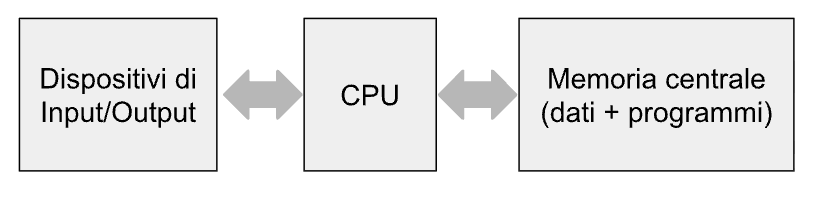
\includegraphics[width=0.5\textwidth]{../images/Vonn Schema.png}
    \caption{Schema di Vonn Neumann}
\end{figure}
La memoria centrale contiene dati da elaborare e programmi, i dispositivi di input e output scambiano dati e interagiscono con il mondo esterno, mentre la CPU esegue le istruzioni di programma (Modello di Von Neumann).
\\La \textbf{CPU} è il cuore del Sistema. Esso esegue programmi scritti in linguaggio macchina (codice nativo), rappresentati come sequenze di byte che codificano istruzioni.
\\I \textbf{Bus} sono strutture di interconnessione che collegano le varie componenti del sistema consentendo lo scambio dei dati. I bus sono canali di comunicazione che trasferiscono i dati a blocchi fissi di byte, chiamati word, che è generalmente di 4 byte oppure 8 byte.
\\L’ \textbf{I/O Bridge} si occupa di coordinare lo scambio dati fra la CPU e il resto del sistema. 
\\I \textbf{Controller e adattatori} interfacciano il sistema verso il mondo esterno, ad esempio acquisendo i movimenti del mouse o i tasti premuti sulla tastiera. La differenza fra i due è che i controller sono saldati sulla scheda madre oppure sono integrati nel dispositivo esterno, mentre gli adattatori sono schede esterne collegate alla scheda madre.
\\Il \textbf{Sistemi di memoria} di un calcolatore è molto articolato. La CPU non comunica direttamente con la memoria principale (RAM), ma ci sono una serie di strati di memorie intermedie chiamate cache che memorizzano i dati più frequentemente acceduti o adiacenti. Le cache hanno tempo di accesso molto inferiori a quelli di una RAM.

\subsection{Elementi di base di un microprocessore}
Negli elementi di base di un processore abbiamo le porte logiche che realizzano funzionalità elementari di una CPU. Le tre porte logiche principali sono: AND, OR, NOT e sono rappresentate dai seguenti simboli:
\begin{figure}[H]
    \centering
    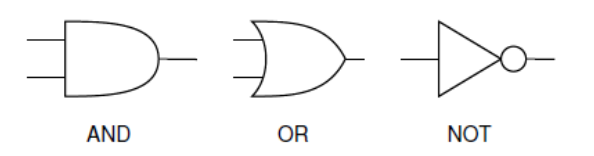
\includegraphics[width=0.5\textwidth]{../images/Porte logiche.png}
    \caption{Porte Logiche}
\end{figure}
Analizziamo una porta alla volta, cominciando dalla porta \textbf{AND}, realizza un operatore binario che vale 1 se e solo se entrambi i propri argomenti sono 1:
\begin{figure}[H]
    \centering
    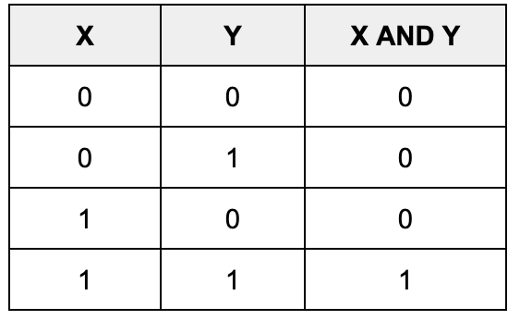
\includegraphics[width=0.5\linewidth]{../images/Tabella AND.png}
    \caption{Tabella Porta Logica AND}
\end{figure}
La porta \textbf{OR} realizza un operatore binario che vale 1 se e solo se almeno uno dei propri argomenti è 1:
\begin{figure}[H]
    \centering
    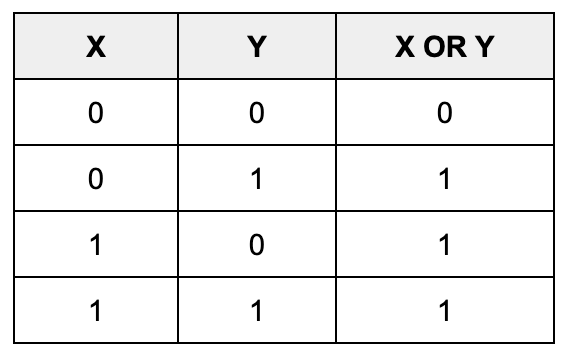
\includegraphics[width=0.5\linewidth]{../images/Tabella OR.png}
    \caption{Tabella Porta Logica OR}
\end{figure}
La porta \textbf{NOT} realizza un operatore unitario che vale 1 se e solo se il proprio argomento è 0:
\begin{figure}[H]
    \centering
    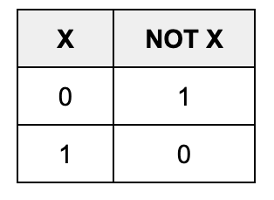
\includegraphics[width=0.2\linewidth]{../images/Tabella NOT.png}
    \caption{Tabella Porta Logica NOT}
\end{figure}
\noindent Abbiamo anche la possibilità di circuiti combinatori che realizzano funzioni booleane arbitrarie, vediamo un esempio di addizionatore parziale:
\begin{figure}[H]
    \centering
    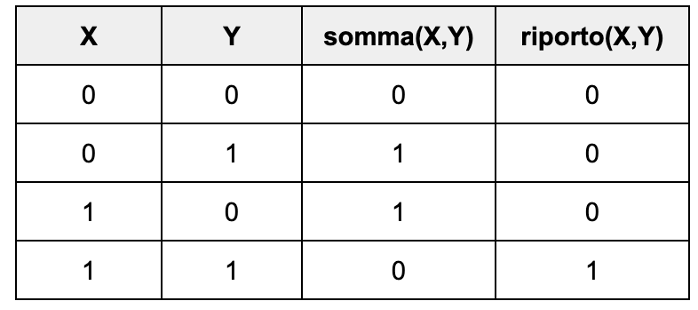
\includegraphics[width=0.5\linewidth]{../images/Tabella Operazioni Logiche.png}
    \caption{Operazioni Logiche}
\end{figure}
\noindent Inoltre un’espressione, gli operatori hanno priorità, dalla maggiore alla minore in questo ordine: NOT, AND, OR.
\newpage
\section{Come viene programmato un Sistema di Calcolo}
\subsection{Linguaggio Alto e Basso Livello}
Nei linguaggi di programmazione possiamo differenziarli in: alto livello e basso livello. Un linguaggio di \textbf{alto livello} forniscono costrutti molto più potenti e sono molto più semplici da imparare, esempi sono: C, Python, ecc.… Programmatori più avanzati prediligono l’uso di linguaggi di \textbf{livello più basso} per avere un codice più ottimizzato per le prestazioni, esempio è il linguaggio Assembly. 
\begin{figure} [H]
    \centering
    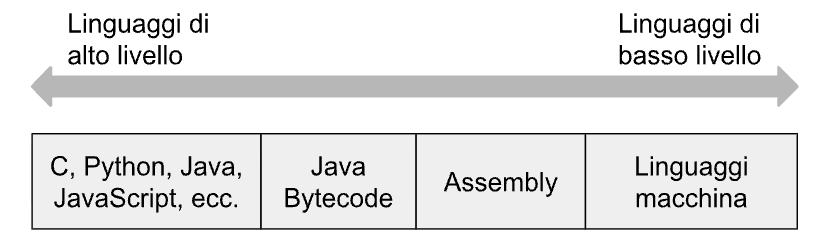
\includegraphics[width=0.5\linewidth]{../images/Linguaggi Livello.png}
    \caption{Classifica Linguaggi}
\end{figure}
\noindent Il linguaggio macchina è un linguaggio particolare progettato con l’obbiettivo di essere facilmente interpretabile dai sistemi elettronici.
\subsection{Compilatori e Interpreti}
C’è da fare ancora una differenziazione tra i linguaggi, di fatto abbiamo due tipi di linguaggi: compilati e interpretati. Nei linguaggi \textbf{compilati} il programma di alto livello viene tradotto in codice macchina in modo da essere eseguito direttamente dalla CPU, questa operazione viene chiamata compilazione; mentre un linguaggio \textbf{interpretato} esegue direttamente il programma senza bisogno di compilarlo prima, questi linguaggi vengono chiamati linguaggi di scripting. Esiste anche la possibilità di avere un linguaggio \textbf{ibrido}, ovvero il programma viene prima compilato in codice scritto in un linguaggio intermedio per poi venire interpretato. Ogni metodologia comporta i vantaggi e svantaggi:
\begin{verbatim}
    Compilati:
\end{verbatim}
\begin{itemize}
    \item Vantaggi $\xrightarrow{}$ il compilatore genera un codice ottimizzato per la piattaforma di calcolo considerata ottenendo migliori prestazioni.
    \item Svantaggi $\xrightarrow{}$ il programma non è portatile, è quindi eseguibile solo sulla piattaforma di calcolo su cui è stata compilata.
\end{itemize}
\begin{verbatim}
    Interpretati:
\end{verbatim}
\begin{itemize}
    \item Vantaggi $\xrightarrow{}$ il programma è portatile, inoltre è possibile eseguirlo direttamente senza bisogno di compilarlo.
    \item Svantaggi $\xrightarrow{}$ l’esecuzione è più lenta, tuttavia alcuni interpreti, come Java Bytecode, utilizzano una tecnica chiamata Just-in-time compilation (JIT) che consiste nel compilare il programma da eseguire in codice nativo subito prima di essere eseguito.
\end{itemize}
\begin{verbatim}
    Ibridi:
\end{verbatim}
\begin{itemize}
    \item Vantaggi $\xrightarrow{}$ programma portabile. 
    \item Svantaggi $\xrightarrow{}$ stessi dei linguaggi interpretati.
\end{itemize}
Noi ci occuperemo del linguaggio C. La compilazione di un programma C può essere scomposta nella compilazione di più moduli C, detti translation unit, ciascuno con estensione “.c”. 
\begin{figure}[H]
    \centering
    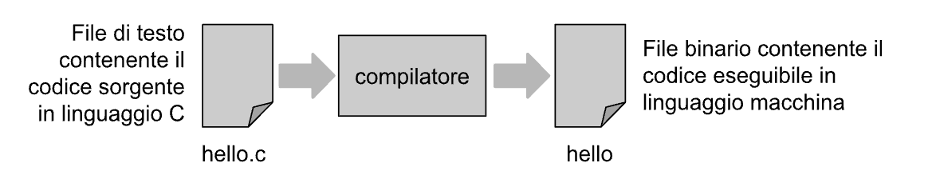
\includegraphics[width=0.5\linewidth]{../images/Funzionamento C.png}
    \caption{Esempio con C}
\end{figure}
\noindent Il processo di compilazione in C è composto in realtà da diversi stadi che vengono effettuati dal sistema di compilazione (compilation toolchain), senza rendercene conto:
\begin{figure}[H]
    \centering
    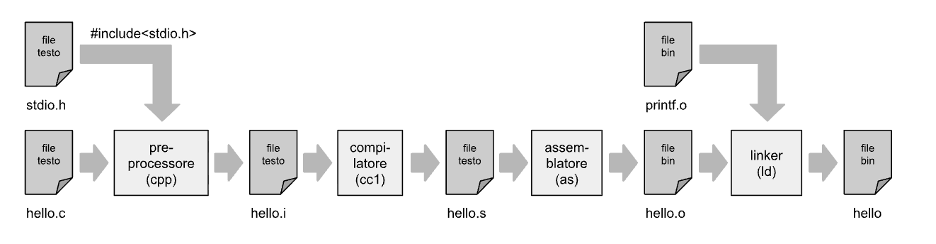
\includegraphics[width=0.7\linewidth]{../images/Funzionamento C2.png}
    \caption{Esempio con C}
\end{figure}
\noindent Gli stadi coinvolgono diversi sottoprogrammi che vengono attivati nel sistema di compilazione:
\begin{itemize}
    \item \textbf{Processore} $\xrightarrow{}$ prende un testo C e lo converte in un altro testo C con le direttive già elaborate (\#include, \#define, ecc…). Quindi oltre che leggere il file “hello.c” leggerà anche il file della libreria “stdio.h”. Per intenderci, il comando: [gcc -E hello.c].
    \item \textbf{Compilatore} $\xrightarrow{}$ prende il testo C senza direttive, verifica la correttezza sintattica e lo traduce in assembly. Con il comando: [gcc -S hello.i].
    \item \textbf{Assembler} $\xrightarrow{}$ prende un programma in assembly e lo traduce in codice macchina generando un file oggetto binario. Tramite: [gcc -c hello.s]
    \item \textbf{Linker} $\xrightarrow{}$ prende i vari file oggetto e li collega insieme a formare un unico file eseguibile. Nel nostro caso collega insieme “hello.o” contenente il codice macchina e “printf.o” contenente il codice macchina che realizza la funzione “printf” invocata dal programma, dando come risultato il file eseguibile “hello”. Con l'utilizzo del comando: [gcc hello.o -o hello].
\end{itemize}
Il collegamento può avvenire in due modi possibili: \textbf{linking statico}, nel quale il codice oggetto della funzione chiamata viene copiato nel file eseguibile, e \textbf{linking dinamico} dove il codice oggetto della funzione chiamata risiede in un file fornito con il sistema operativo, successivamente il collegamento tra la chiamata a funzione ed il codice che lo implementa viene fatto al caricamento del file eseguibile. Esisto in realtà un altro tipo di collegamento di linking  chiamato \textbf{linking a Runtime}, che avviene durante l’esecuzione del programma, il collegamento tra programma e le librerie necessarie viene effettuato solo nel momento in cui serve realmente quella funzione, mentre il programma è già in funzione, permette di caricare le librerie solo quando necessario.
\\Nei programmi possiamo riscontrare tipi diversi di errore, come gli \textbf{errori in fase di esecuzione} (Runtime) che rappresentano problemi che si verificano mentre il programma è in funzione, spesso dovuto all’incompatibilità tra parte software (programma) e hardware oppure a operazioni non valide. Esempio è la divisione per 0. 
\\Abbiamo inoltre anche gli \textbf{errori in fase di compilazione} che si verificano durante la fase di compilazione, causati da errori di sintassi o di scrittura del codice, come parentesi mancanti, variabili non dichiarati ecc.,  e impediscono al programma di avviarsi finché non vengono corretti.
\\ \textbf{Instruction set architecture} (ISA) ed è lo standard che definisce come funziona una struttura di calcolo, in modo più preciso un processore. All’interno del documento possiamo trovare:
\begin{itemize}
    \item \textit{Stato della CPU}
    \begin{itemize}
        \item Registri $\xrightarrow{}$ quanti e quali. 
        \item Memoria
    \end{itemize}
    \item \textit{Istruzioni}
    \begin{itemize}
        \item Formato
        \item Tipologie $\xrightarrow{}$ spostamento dati, aritmetico/logiche, controllo.
    \end{itemize}
    \item \textit{Semantica delle istruzioni} $\xrightarrow{}$ come l’esecuzione di ciascuna istruzione modifica lo stato.
\end{itemize}

\subsection{Formato testo, oggetto ed eseguibile}
Il formato binario ELF (Executable and Linkable Format) è un tipo di formato usato nei sistemi operativi per i file eseguibili, le librerie e i file oggetto. Contiene diverse parti tra cui:
\begin{itemize}
    \item Informazioni sul programma
    \item Codice da eseguire
    \item Dati del programma
    \item Informazioni per il collegamento con librerie esterne
\end{itemize}
Non può essere eseguito o linkato su MacOS X. Allo stesso modo un file formato Mach-O non può essere eseguito o linkato in Linux; pertanto, i formati eseguibili non garantiscono la portabilità dei programmi.
\subsection{Disassemblare programmi in codice macchina: objdump}
Disassemblare un programma in linguaggio macchina consiste nel tradurne le istruzioni nel codice assembly corrispondente in modo che possano essere analizzate da un programmatore. 
\begin{figure} [H]
    \centering
    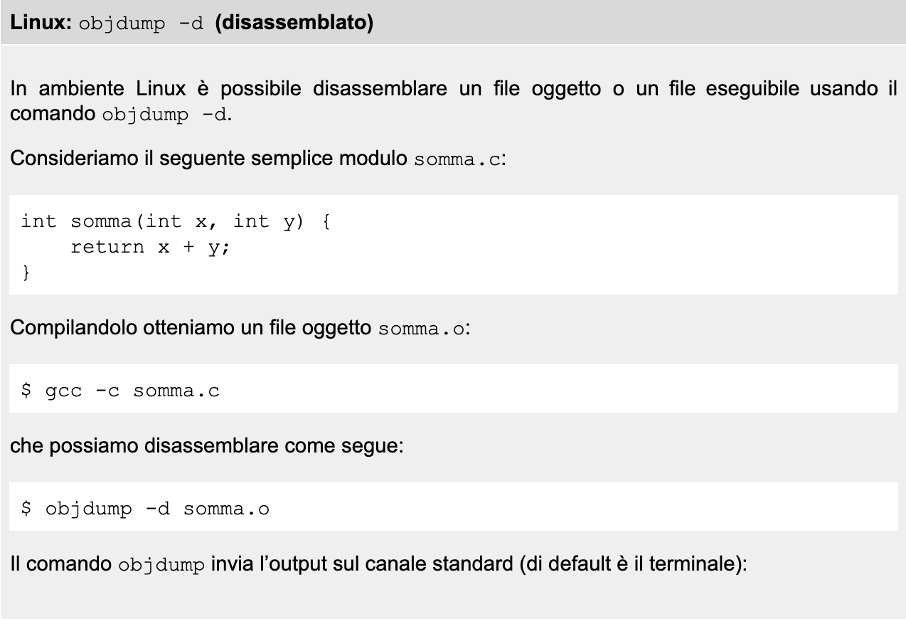
\includegraphics[width=0.7\linewidth]{../images/Objdump Esempio.png}
    \caption{Esempio Objdump}
\end{figure}
\subsection{Traduzione in linguaggio macchina programma C}
I sistemi di calcolo si basano su un certo numero di astrazioni che forniscono una visione più semplice del funzionamento della macchina. Due delle più importanti astrazioni sono:
\begin{itemize}
    \item \textbf{Memoria} $\xrightarrow{}$ vista come un grosso array di byte
    \item \textbf{ISA} (Instruction Set Architecture) $\xrightarrow{}$ definisce:
    \begin{itemize}
        \item Stato della CPU
        \item Formato delle sue istruzioni
        \item Effetto che le istruzioni hanno sullo stato
    \end{itemize}
\end{itemize}
\begin{figure} [H]
    \centering
    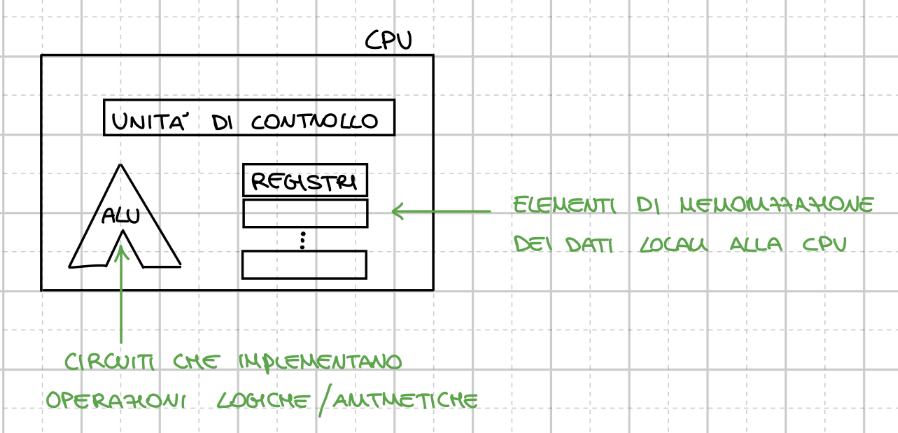
\includegraphics[width=0.5\linewidth]{../images/ALU.png}
    \caption{ALU}
\end{figure}
Per tradurre codice di alto livello in codice macchina, i compilatori si basano sulla descrizione astratta della macchina data dalla sua ISA. Le più diffuse sono:
\begin{itemize}
    \item \textbf{IA32} $\xrightarrow{}$ -	IA32 → A, B, C, D, DI, SI, BP, SP, EP, IP, EFLAGS, i primi 7 sono general purpose, ovvero possono essere utilizzati a piacimento seguendo comunque le regole. \textbf{BP e SP} fanno parte della gestione dello stack. Abbiamo poi il registro \textbf{IP} (Instruction Pointer) è un registro non modificabile ma solo leggibile che viene gestito in maniera automatica dalla CPU, inserendo l’indirizzo della prossima istruzione da eseguire in memoria. Infine, abbiamo \textbf{EFLAGS}, anch’esso non modificabile che contiene dei flag che descrivono lo stato di funzionamento della CPU. Ciascun registro contiene 32 bit, così distribuiti:
\end{itemize}
\begin{figure} [H]
    \centering
    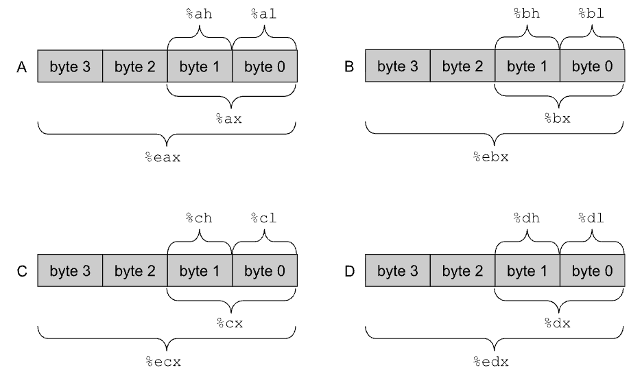
\includegraphics[width=0.7\linewidth]{../images/IA32 Registri.png}
    \caption{Registri IA32}
\end{figure}
Mentre gli altri registri hanno una suddivisione leggermente diversa:
\begin{figure} [H]
    \centering
    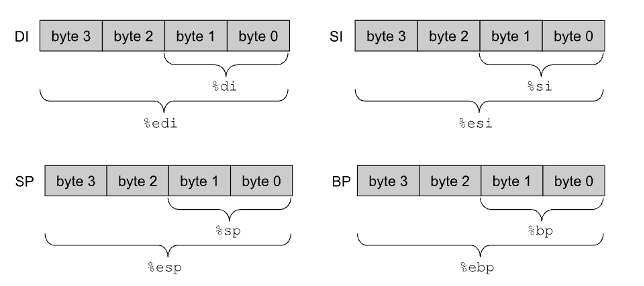
\includegraphics[width=0.7\linewidth]{../images/Registri IA32 2.png}
    \caption{Registri IA32}
\end{figure}
\noindent I tipi macchina permettono di rappresentare sia numeri interi che numeri con virgola mobile. Vediamo in cosa corrispondono in C:
\begin{figure} [H]
    \centering
    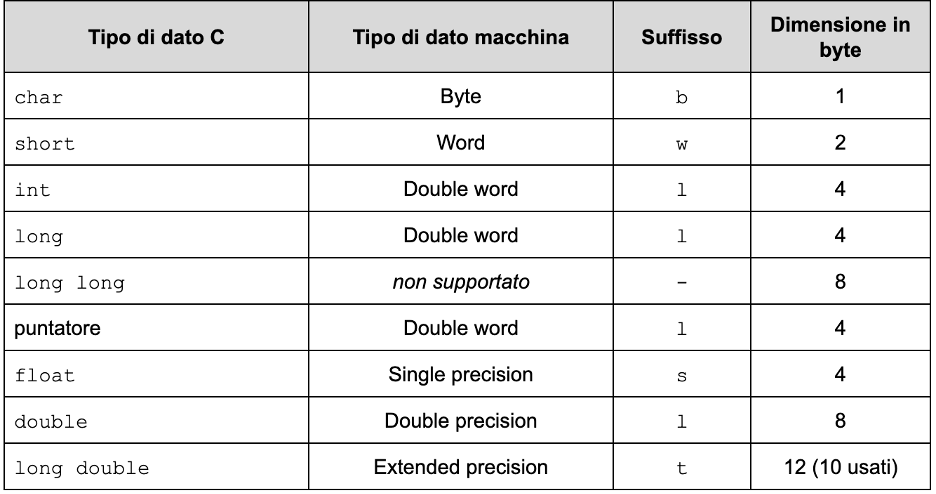
\includegraphics[width=0.5\linewidth]{../images/Tipi di dati convertiti.png}
    \caption{Tipi di Dati}
\end{figure}
\begin{itemize}
    \item \textbf{X86-64} $\xrightarrow{}$ descrive le architetture della famiglia di processori x86 a 64 bit, è retrocompatibile con IA32, ovvero le istruzioni di IA32 sono presenti anche nell’x86-64.
\end{itemize}
Si hanno 11 possibili forme di operandi. Per gli operandi di memoria, ci sono vari modi di indirizzamento che consentono di accedere alla memoria dopo averne calcolato un indirizzo:
\begin{table}[H]
    \centering
    \begin{tabular}{|c|c|c|c|}
        \hline
        \textbf{Tipo} & \textbf{Sintassi} & \textbf{Valore Denotato} & \textbf{Nome Convenzionale} \\
        \hline
        \textit{Immediato} & \$imm & imm & immediato \\
        \hline
        \textit{Registro} & E & R[E] & Registro \\
        \hline
        \textit{Memoria} & imm & M[imm] & Assoluto\\
        \hline
        \textit{Memoria} & $E_{base}$ & M[R[$E_{base}$]] & Indiretto\\
        \hline
        \textit{Memoria} & imm($E_{base}$) & M[imm+R[$E_{base}$]] & Base e spiazzamento\\
        \hline
        \textit{Memoria} & ($E_{base}$,$E_{indice}$) & M[imm+R[$E_{base}$]+R[$E_{indice}$]] & Base e indice\\
        \hline
        \textit{Memoria} & imm($E_{base}$,$E_{indice}$) & M[imm+R[$E_{base}$]+R[$E_{indice}$]] & Base, indice e spiazzamento \\
        \hline
        \textit{Memoria} & ($E_{indice}$,s) & M[R[$E_{indice}$]] $\cdot$ s] & Indice e scala \\
        \hline
        \textit{Memoria} & imm($E_{indice}$,s) & M[imm+R[$E_{indice}$] $\cdot$ s] & Base, indice, scala e spiazzamento \\
        \hline
        \textit{Memoria} & imm($E_{base}$,$E_{indice}$,s) & M[R[$E_{base}$]+R[$E_{indice}$] $\cdot$ s] & Base, indice e scala\\
        \hline
        \textit{Memoria} & imm($E_{base}$,$E_{indice}$,s) & M[imm+R[$E_{base}$]+R[$E_{indice}$] $\cdot$ s] & Base, indice, scala e spiazzamento \\
        \hline
    \end{tabular}
    \caption{Operandi Possibili}
\end{table}
\noindent Abbiamo anche due modi in cui un processore definisce l’ordine in cui vengono disposti in memoria i byte della rappresentazione di un valore numerico (binari):
\begin{itemize}
    \item \textbf{Big-Endian} $\xrightarrow{}$ il bit più significativo viene posto all’indirizzo più basso.
    \item \textbf{Big-Endian} $\xrightarrow{}$ il bit meno significativo viene posto all’indirizzo più basso.
\end{itemize}
\begin{figure}[H]
    \centering
    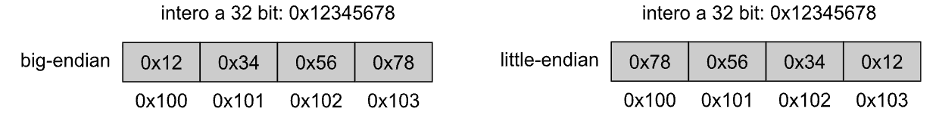
\includegraphics[width=0.5\linewidth]{../images/Big E Little Endian.png}
    \caption{Big e Little Endian}
\end{figure}
L’architettura di IA32 è Little-Endian, mentre sono Big-Endian PowerPC e SPARC.
\\Noi per il momento utilizzeremo i registri A, C, D.

